\documentclass[12pt]{article}
\usepackage[margin=1in]{geometry} 
\usepackage{amsmath,amsthm,amssymb,amsfonts,bbm}
\usepackage[utf8]{inputenc}
\usepackage[english]{babel}
\usepackage{hyperref}
\usepackage{tikz}
\usetikzlibrary{trees}
\usetikzlibrary{matrix}

\newcommand{\N}{\mathbb{N}}
\newcommand{\Z}{\mathbb{Z}}

\newenvironment{Exercise}[2][Exercise]{\begin{trivlist}
		\item[\hskip \labelsep {\bfseries #1}\hskip \labelsep {\bfseries #2.}]}{\end{trivlist}}
\newenvironment{Lemma}[2][Lemma]{\begin{trivlist}
		\item[\hskip \labelsep {\bfseries #1}\hskip \labelsep {\bfseries #2.}]}{\end{trivlist}}
%If you want to title your bold things something different just make another thing exactly like this but replace "problem" with the name of the thing you want, like theorem or lemma or whatever
\newtheorem{theorem}{Theorem}[section]
\newtheorem{corollary}{Corollary}[theorem]
\newtheorem{lemma}{Lemma}
\begin{document}

	
	\title{State Prices}
	\author{Peiliang Guo}
	\maketitle
	\begin{Exercise}{1}	\end{Exercise}
	\begin{proof}
		(i) Follows from $\mathbb{P}(\omega)>0$ for all $\omega$\\
		(ii) $$\tilde{\mathbb{E}}\frac{1}{Z} = \sum_{\omega\in\Omega}\frac{\mathbb{P}(\omega)}{\tilde{\mathbb{P}}(\omega)}\tilde{\mathbb{P}}(\omega) = \sum_{\omega\in\Omega}\mathbb{P}(\omega) = 1$$
		(iii) $$\mathbb{E}Y = \sum_{\omega\in\Omega}Y(\omega)\mathbb{P}(\omega) = \sum_{\omega\in\Omega}Y(\omega)\frac{\mathbb{P}(\omega)}{\tilde{\mathbb{P}}(\omega)}\tilde{\mathbb{P}}(\omega)=\sum_{\omega\in\Omega}Y(\omega)\cdot\frac{1}{Z(\omega)}\tilde{\mathbb{P}}(\omega) = \tilde{\mathbb{E}}\left[\frac{1}{Z}\cdot Y\right]$$
	\end{proof}
	\begin{Exercise}{2} \end{Exercise}
	\begin{proof}
	(i) $$\tilde{\mathbb{P}}(\Omega)=\sum_{\omega\in\Omega}\tilde{\mathbb{P}}(\omega)=\sum_{\omega\in\Omega}Z(\omega)\mathbb{P}(\omega) = \mathbb{E}[Z] = 1$$
	\end{proof}
	(ii) $$\tilde{\mathbb{E}}Y = \sum_{\omega\in\Omega}Y(\omega)\tilde{\mathbb{P}}(\omega) = \sum_{\omega\in\Omega} Y(\omega) Z(\omega)\mathbb{P}(\omega)=\mathbb{E}[YZ]$$
	(iii) Since $\mathbb{P}(A) = 0$, then $\mathbb{P}(\omega) = 0$ for all $\omega\in A$. 
	$$\tilde{\mathbb{P}}(A) = \sum_{\omega\in A} \tilde{\mathbb{P}}(\omega) = \sum_{\omega\in A} Z(\omega)\mathbb{P}(\omega) = 0$$
	(iv) Since $\mathbb{P}(Z>0) = 1$, $\mathbb{P}(Z=0)  = 0$, i.e. for all $\omega \in\Omega$ such that $Z(\omega)=0$, $\mathbb{P}(\omega) = 0$. 
	$$0 = \tilde{\mathbb{P}}(A) =\sum_{\omega\in A}Z(\omega)\mathbb{P}(\omega) = \sum_{\omega\in A, Z(\omega)=0}Z(\omega)\mathbb{P}(\omega)+ \sum_{\omega\in A, Z(\omega)>0}Z(\omega)\mathbb{P}(\omega)= \sum_{\omega\in A, Z(\omega)>0}Z(\omega)\mathbb{P}(\omega)$$
	This forces for all $\omega\in A$ such that $Z(\omega)>0$, $\mathbb{P}(\omega)=0$. Therefore, 
	$$\mathbb{P}(A) = \sum_{\omega\in A}\mathbb{P}(\omega) = \sum_{\omega\in A, Z(\omega)>0}\mathbb{P}(\omega) + \sum_{\omega\in A, Z(\omega)=0}\mathbb{P}(\omega) = 0$$
	(v) $$\mathbb{P}(A) = 1 \iff \mathbb{P}(A^c) = 0 \iff \tilde{\mathbb{P}}(A^c) = 0 \iff \tilde{\mathbb{P}}(A) = 1$$
	(vi) Suppose we have $\mathbb{P}(H) = \frac{1}{2}$ and $\mathbb{P}(T) = \frac{1}{2}$, and if $Z(H)=2$ and $Z(T) = 0$, then we have  $\mathbb{P}(Z\ge 0) = 1$ and $\tilde{\mathbb{P}}(H) = 2\cdot\frac{1}{2} = 1$ and $\tilde{\mathbb{P}}(T) = 0 \cdot \frac{1}{2} = 0$ which is not equivalent to $\mathbb{P}$. 
	\begin{Exercise}{3} \end{Exercise}
	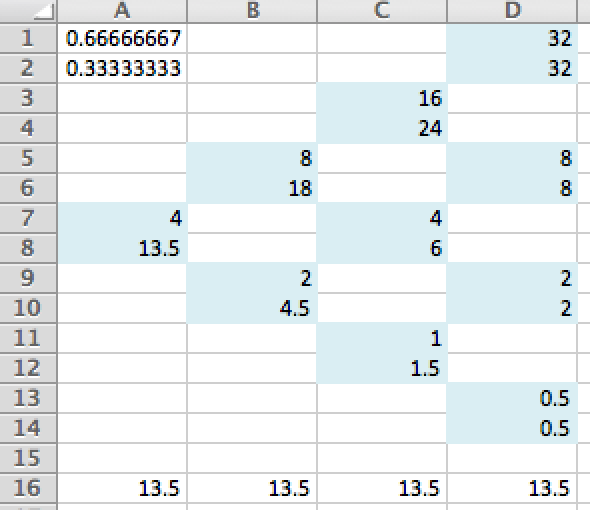
\includegraphics{Ex3_3.png}
	\begin{Exercise}{4} \end{Exercise}
	(i) 
	\begin{align*}
	\zeta_3(HHH) &= \frac{1}{(1+\frac{1}{4})^3}\frac{27}{64}=\frac{27}{125}\\
	\zeta_3(HHT) &= \zeta_3(HTH) = \zeta_3(THH) = \frac{1}{(1+\frac{1}{4})^3}\frac{27}{32}=\frac{54}{125}\\
	\zeta_3(HTT) &= \zeta_3(THT) = \zeta_3(TTH) = \frac{1}{(1+\frac{1}{4})^3}\frac{27}{16}=\frac{108}{125}\\
	\zeta_3(TTT) &= \frac{1}{(1+\frac{1}{4})^3}\frac{27}{8}=\frac{216}{125}\\
	\end{align*}
	(ii) $$V_0 = \sum_{\omega\in\Omega}V_N(\omega)\zeta(\omega)\mathbb{P}(\omega)$$
	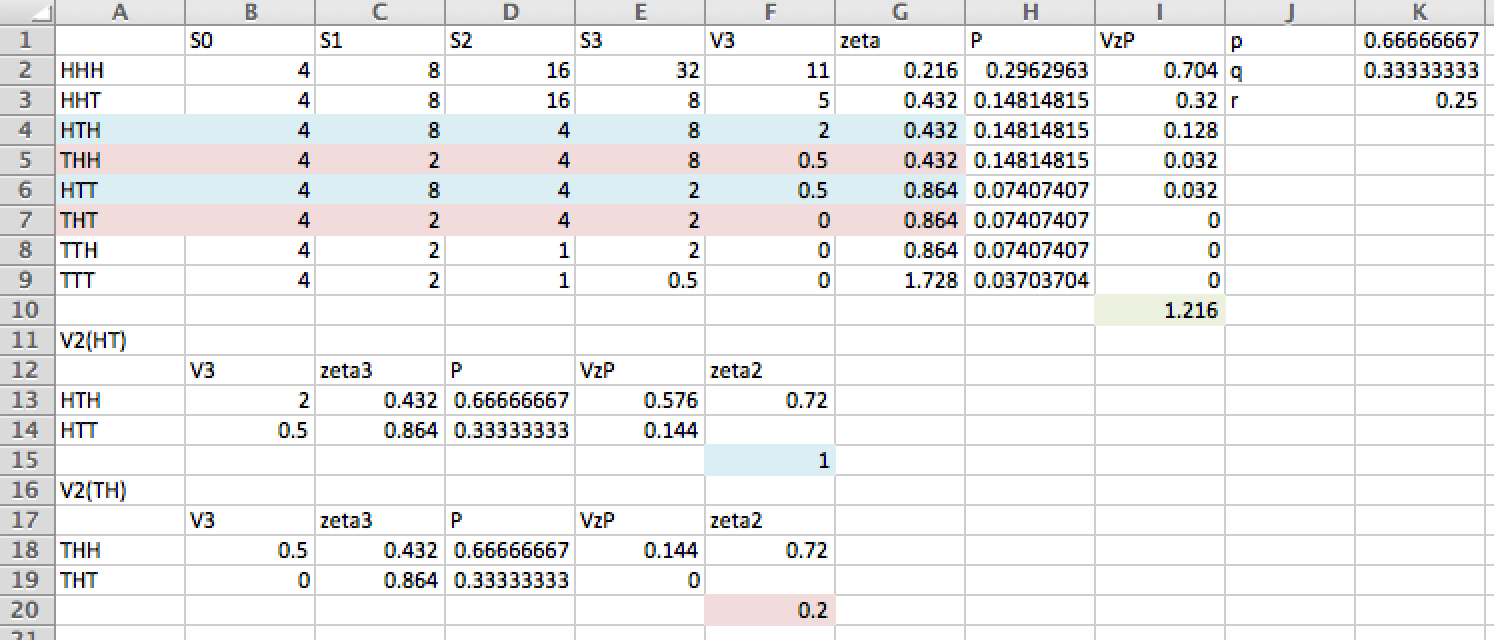
\includegraphics[scale=0.6]{Ex3_4.png}\\
	(iii) $\zeta_2(HT)=\zeta_2(TH)=\frac{1}{(1+r)^2}Z(TH)=\frac{1}{(1+r)^2}Z(HT)=\frac{1}{(1+\frac{1}{4})^2}\frac{9}{8}=\frac{18}{25}$\\
	(iv) 
	\begin{align*}
	V_2(HT)&=\frac{1}{\zeta_2(HT)}\mathbb{E}_2[\zeta_3V_3](HT)=\frac{25}{18}\left(\frac{2}{3}\cdot 0.432\cdot 2+\frac{1}{3}\cdot 0.864\cdot 0.5\right)=1\\
	V_2(TH)&=0.2
	\end{align*}
	\begin{Exercise}{5} \end{Exercise}
	(i)
	\begin{align*} 
	Z(HH) &= \frac{\tilde{\mathbb{P}}(HH)}{\mathbb{P}(HH)} = \frac{\frac{1}{4}}{\frac{4}{9}}=\frac{9}{16}\\
	Z(HT) &= \frac{\tilde{\mathbb{P}}(HT)}{\mathbb{P}(HT)} = \frac{\frac{1}{4}}{\frac{2}{9}}=\frac{9}{8}\\
	Z(TH) &= \frac{\tilde{\mathbb{P}}(TH)}{\mathbb{P}(TH)} = \frac{\frac{1}{12}}{\frac{2}{9}}=\frac{3}{8}\\
	Z(TT) &= \frac{\tilde{\mathbb{P}}(TT)}{\mathbb{P}(TT)} = \frac{\frac{5}{12}}{\frac{1}{9}}=\frac{15}{4}\\
	\end{align*}
	(ii)
	\begin{align*}
	Z_1(H) &= \mathbb{E}_1[Z](H)=p Z(HH)+qZ(HT) = \frac{2}{3}\cdot\frac{9}{16}+\frac{1}{3}\cdot\frac{9}{8}=\frac{3}{4}\\
	Z_1(T) &= \mathbb{E}_1[Z](T)=p Z(TH)+qZ(TT) = \frac{2}{3}\cdot\frac{3}{8}+\frac{1}{3}\cdot\frac{15}{4}=\frac{3}{2}\\
	\text{Note that }Z_0 &= pZ(H)+qZ(T)=\frac{2}{3}\cdot\frac{3}{4}+\frac{1}{3}\cdot\frac{3}{2}=1
	\end{align*}
	(iii)
	\begin{align*}
		V_1(H)&=\frac{1+r_0}{Z_1(H)}\mathbb{E}_1\left[\frac{Z_2}{(1+r_0)(1+r_1)}V_2\right](H)\\
			&=\frac{1}{Z_1(H)(1+r_1(H))}\mathbb{E}_1[Z_2V_2](H)\\
			&=\frac{1}{\frac{3}{4}(1+\frac{1}{4})}\cdot\left(\frac{2}{3}\frac{9}{16}\cdot 5+\frac{1}{3}\frac{9}{8}\cdot 1\right)\\
			&=\frac{12}{5}\\
		V_1(T)&=\frac{1}{Z_1(T)(1+r_1(T))}\mathbb{E}_1[Z_2V_2](T)\\
			&=\frac{1}{\frac{3}{2}(1+\frac{1}{2})}\cdot\left(\frac{2}{3}\frac{3}{8}\cdot 1\right)\\
			&=\frac{1}{9}\\
		V_0 &= \mathbb{E}\left[\frac{Z_2}{(1+r_0)(1+r_1)}V_2\right]\\
			&=\left(\frac{4}{9}\frac{\frac{9}{16}}{(1+\frac{1}{4})(1+\frac{1}{4})}\cdot 5\right)+\left(\frac{2}{9}\frac{\frac{9}{8}}{(1+\frac{1}{4})(1+\frac{1}{4})}\cdot 1\right)+\left(\frac{2}{9}\frac{\frac{3}{8}}{(1+\frac{1}{4})(1+\frac{1}{2})}\cdot 1\right)\\
			&=\frac{236}{225}
	\end{align*}
 \end{document}

	